%-------------------------------------------------------------------------------
%-------------------------------------------------------------------------------
\chapter{Introduction}
%-------------------------------------------------------------------------------
%-------------------------------------------------------------------------------
\thispagestyle{empty}
%-------------------------------------------------------------------------------
%-------------------------------------------------------------------------------
\begin{abstract} Dans ce T.P. nous allons prendre contact avec l'environnement de travail utilisé durant l'année et expérimenter quelques ressources de python. Une grande partie des exercices seront approfondis durant le déroulement de l'année.

Pendant tous les T.P. il est capital de ne jamais rester passif : essayez, lisez les documentations, posez des questions à vos enseignants ou à ceux de vos camarades qui sont les plus rapides.
\end{abstract}
%-------------------------------------------------------------------------------
%-------------------------------------------------------------------------------
%-------------------------------------------------------------------------------
%-------------------------------------------------------------------------------
%-------------------------------------------------------------------------------
\section{Écosystème} 
%-------------------------------------------------------------------------------
%-------------------------------------------------------------------------------
%-------------------------------------------------------------------------------
Nous utiliserons des outils dans un environnement qui sera, selon les séances, Windows ou Linux. Leurs fonctionnalités sont semblables mais il est utile de se familiariser avec chacun d'eux.

Pour utilisez les ordinateurs vous devez vous connecter avec votre identifiant (nom.prénom) et votre mot de passe. Le mot de passe initial est votre date de naissance et il {\bf doit} être changé\footnote{Cela n'est possible que sur les ordinateurs sous Windows.}.
%-------------------------------------------------------------------------------
%-------------------------------------------------------------------------------
\subsection{Répertoires et fichiers}
%-------------------------------------------------------------------------------
%-------------------------------------------------------------------------------
\begin{center}
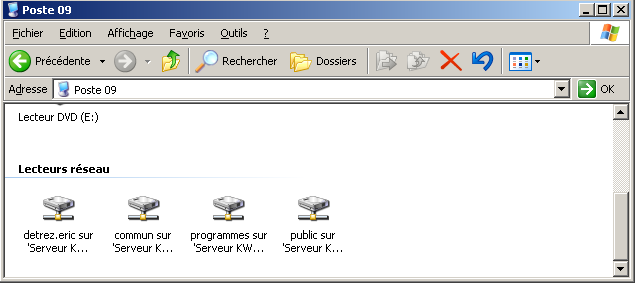
\includegraphics[scale=0.5]{01_disques.png} 
\end{center}
%-------------------------------------------------------------------------------
Il y a 4 dossiers distants accessibles : Commun, Public, Programmes et votre dossier personnel, à votre nom.
%-------------------------------------------------------------------------------
\begin{itemize}

\item Sous Windows ils sont visibles comme des lecteurs réseaux, repérés par une lettre

\item Sous Linux ce sont des répertoires.

\end{itemize}
%-------------------------------------------------------------------------------
Chacun a des modalités d'accès propres donc un usage spécifique.
%-------------------------------------------------------------------------------
\begin{itemize}

\item Votre dossier personnel est le plus important. Vous seul y avez accès\footnote{L'administrateur du réseau aussi.} en lecture (vous pouvez lire ce qui y est) et en écriture (vous pouvez y sauvegarder des fichiers). Les fichiers y seront conservés {\bf toute l'année scolaire}. Il ne faut pas le confondre avec le dossier local de votre poste ; dans celui-ci aussi vous pouvez lire et écrire mais les données peuvent être effacées.

\item Le dossier {\bf public} est accessible à toute la classe, les étudiants y ont accès en lecture, les enseignants en lecture et en écriture. C'est le dossier dans lequel les enseignants peuvent transmettre des documents.

\item Le dossier {\bf commun} est accessible à toute la classe en lecture et en écriture. C'est le dossier dans lequel vous pouvez partager des documents avec les autres.

\item Le dossier {\bf programmes} contient des programmes (windows) qui peuvent être lancés. Il permet d'utiliser des programmes sur un poste windows sans qu'il soit installé sur le poste.

\end{itemize}
%-------------------------------------------------------------------------------

{\bf N.B.} La taille totale des fichiers que vous pouvez sauvegarder est limitée (60 Mo) ; évitez les fichiers trop gros (films, musique, ...)

%-------------------------------------------------------------------------------
{\it Créez un répertoire pour l'informatique dans votre dossier, entraînez-vous à y créer des sous-répertoires pour chaque TP.}

%-------------------------------------------------------------------------------
%-------------------------------------------------------------------------------
\section{Présentation de python}
%-------------------------------------------------------------------------------
%-------------------------------------------------------------------------------
\subsection{La boucle interactive}
%-------------------------------------------------------------------------------
Le moyen le plus immédiat d'utiliser python est la boucle interactive lancée depuis un terminal.
%-------------------------------------------------------------------------------
\begin{itemize}

\item On peut trouver un terminal adapté, \type{winpython.exe} dans le dossier \type{Pyzo}
%-------------------------------------------------------------------------------
\begin{center}
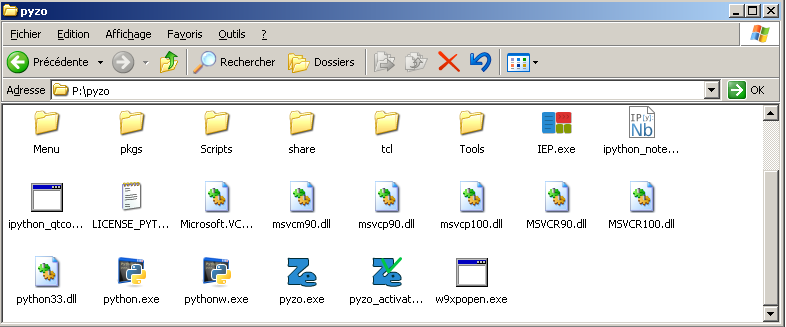
\includegraphics[scale=0.5]{01_cmdwin.png} 
\end{center}
%-------------------------------------------------------------------------------
\item Sur les postes Linux on ouvre le terminal par un clic droit sur un dossier "Ouvrir un terminal ici" puis on tape \type{python}. Python a eu une évolution importante en passant de la version 2 à la version 3 : une version 2.7 subsiste encore parfois mais nous utiliserons python3. Dans le cas où on aurait plusieurs versions de Python installées (2 et 3) on lance Python3 avec la commande \type{python3}.

À notre niveau les différences ne sont pas nombreuses : la plus visible est que \type{print} est devenu une fonction et nécessite que ses arguments soient passés entre parenthèses.

\end{itemize}
%-------------------------------------------------------------------------------
Le programme python attend nos instructions et répond immédiatement.

On peut faire exécuter quelques instructions simples :  \type{2 + 2}, \dots
%-------------------------------------------------------------------------------
\begin{center}
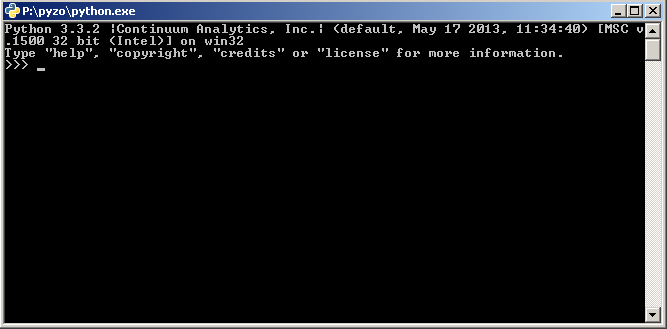
\includegraphics[scale=0.5]{01_winpython.png} 
\end{center}
%-------------------------------------------------------------------------------
On voit ici une particularité de python : c'est un langage interprété.
Cela signifie qu'il ne fabrique pas, avec nos instructions, un programme autonome comme le font d'autres langages comme C ou Pascal. Il traduit nos commandes et les fait exécuter directement par l'ordinateur.

L'avantage est que l'on teste très facilement les programmes, l'inconvénient est qu'on a toujours besoin de python et qu'il lui faut tout traduire à chaque fois qu'on a besoin de notre programme.

On peut néanmoins lancer une suite d'instructions en python (un script) directement : on l'exécute par la commande \type{python "nom\_du\_fichier\_avec\_chemin"}.
%-------------------------------------------------------------------------------
%-------------------------------------------------------------------------------
\subsection{Limitations}
%-------------------------------------------------------------------------------
%-------------------------------------------------------------------------------
Cette boucle interactive est un peu primitive, 

\begin{itemize}
\item il est difficile de gérer des programmes de plus d'une ligne (nous écrirons des programmes d'une dizaine de ligne),
\item en particulier il sera difficile de corriger une erreur,
\item on ne garde pas de trace de ce qui a été écrit.
\end{itemize}

Il existe une boucle interactive améliorée, souvent installée par défaut, \type{iPython}. Il y a une version autonome {\bf iPython qtConsole} qui se lance dans une fenêtre, il existe aussi une version {\bf notebook} qui se lance dans un navigateur. 
%
% \begin{center}
% \includegraphics[scale=0.5]{01_ipython.png} 
% \end{center}
Vous trouverez sur internet des cours qui utilisent cette version.

\medskip

Cependant la méthode la plus générale de programmation consiste à écrire le code dans un éditeur puis à le faire compiler  ou interpréter par le langage. Dans le cas de l'interprétation d'un langage interactif l'interprétation peut se faire de manière accumulative : chaque nouveau code est ajouté et on enrichit petit à petit les outils qui sont à notre disposition. 

Cette dernière méthode est possible dans Python.

On travaillera donc sous la forme d'un va-et-vient entre les instruction dans l'éditeur et leurs interprétations dans la console.

Il existe de nombreux logiciels qui intègrent un éditeur et une console Python, on parle d'{\bf environnements de développement intégrés} ou IDE en anglais, pour Integrated Development Environment.

On trouve des IDE spécifiques à Python.
\begin{itemize}
\item {\bf Pyzo} est utilisé par les oraux de Centrale, c'est celui qui a été choisi dans ce lycée.
\item {\bf Spyder} est assez semblable à Pyzo, certains le préfèrent.
\item {\bf idle} est souvent installé par défaut, il est utilisé à l'oral de l'ENSAM.
\item {\bf Thonny} est un outil à l'aspect épuré mais qui permet une installation facile des modules. De plus son mode de suivi de l'exécution (debug) est très instructif.
\end{itemize}

Les IDE généralistes (netBeans, Eclipse, Sublime Text, Atom, Visual Studio) peuvent être utilisés avec Python.

Les éditeurs de texte ont souvent, nativement ou à l'aide de greffons, la possibilité de travailler directement avec Python : emacs, gedit, notepad++ (windows), textmate (mac) \dots
%-------------------------------------------------------------------------------
%-------------------------------------------------------------------------------
%-------------------------------------------------------------------------------
\section{Pyzo}
%-------------------------------------------------------------------------------
%-------------------------------------------------------------------------------
%-------------------------------------------------------------------------------
\subsection{Présentation}
%-------------------------------------------------------------------------------
%-------------------------------------------------------------------------------
La fenêtre initiale de Pyzo contient plusieurs parties :
%-------------------------------------------------------------------------------
\begin{itemize}
\item la console, [A], c'est l'interpréteur comme vu ci-dessus
\item l'éditeur, [B], qui permet d'écrire les programmes et de les modifier
\item des fenêtres d'utilitaires, [C], qui nous n'utiliserons pas pour l'instant.
\end{itemize}

%-------------------------------------------------------------------------------
\begin{center}
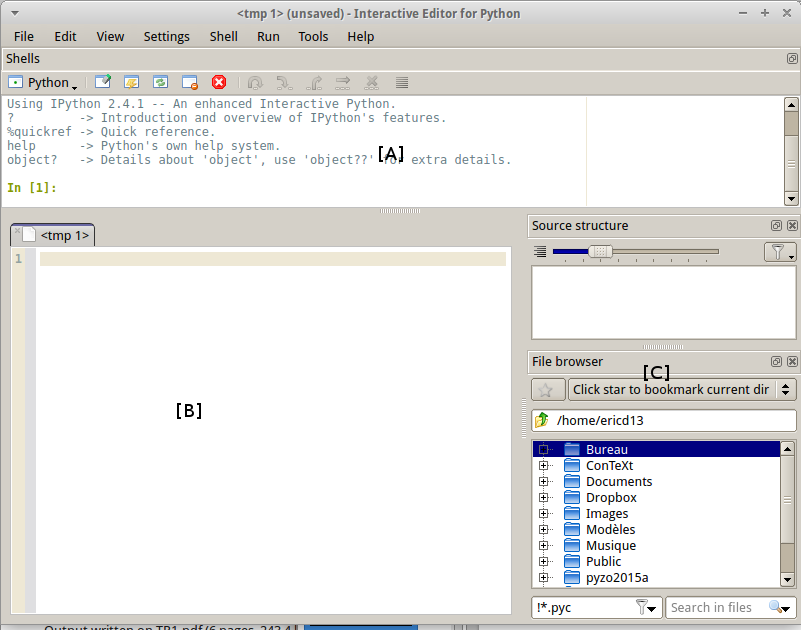
\includegraphics[scale=0.350]{01_Pyzo1.png} 
\end{center}
%-------------------------------------------------------------------------------
%-------------------------------------------------------------------------------
On peut déplacer les composantes, sauf celle de l'éditeur, et fermer les outils qui ne sont pas utiles ; on pourra les retrouver en les ouvrant dans le menu {\bf Outils}

Il est indispensable d'employer l'éditeur dès que l'on veut rentrer plusieurs lignes afin d'obtenir un résultat.               

Il est par ailleurs recommandé que le fichier écrit dans l'éditeur soit complet :
%-------------------------------------------------------------------------------
\begin{enumerate}
\item on commence par les importations ; il n'est pas gênant qu'elles soit répétées, python ne les effectue qu'une fois

\item on poursuit par les différentes fonctions 

\item on finit par les lignes principales qui appliquent ces fonctions.

\end{enumerate}
%-------------------------------------------------------------------------------
On pourra utiliser un fichier-squelette à garder dans son répertoire.

Exemple (ce qui suit le caractère \# n'est pas lu par Python).

\begin{lstlisting}
# Importations


# Fonctions


# Programme principal
\end{lstlisting}

Par ailleurs il vaut mieux faire un fichier par exercice et il est \textbf{indispensable} de les sauvegarder régulièrement.
%-------------------------------------------------------------------------------
%-------------------------------------------------------------------------------
\subsection{Le premier programme}
%-------------------------------------------------------------------------------
%-------------------------------------------------------------------------------
Dans la fenêtre de l'éditeur effacer les lignes déjà écrites et écrire le programme le plus employé pour un premier exemple :

\begin{lstlisting}
print("Hello World")
\end{lstlisting}
%-------------------------------------------------------------------------------
\begin{itemize}
\item On commence par sauvegarder le fichier en choisissant un emplacement que l'on peut retrouver et qui garde les données, le plus simple est le répertoire personnel du serveur du lycée que l'on peut lire partout dans le lycée.

\item Il faut maintenant faire exécuter le fichier dans la console python

\begin{itemize}
\item soit par un item  \textit{Exécuter le fichier} du menu \textit{Exécuter}

\item soir par un raccourci ([F5] ou [Ctrl]+[Entrée])
\end{itemize}


\item Tout se passe presque comme si on avait écrit les instructions dans la console.

\end{itemize}
%-------------------------------------------------------------------------------
\begin{center}
\fbox{\begin{minipage}{0.9\linewidth}
Rappel : il est indispensable de sauvegarder régulièrement son travail. Pour cela il faut utiliser le raccourci-clavier [Ctrl] + S : on appuie sur la touche [Ctrl] puis, tout en maintenant l'appui sur [Ctrl], on appuie sur la touche S. On peut alors relâcher les deux touches.
\end{minipage}}
\end{center}
%-------------------------------------------------------------------------------
%-------------------------------------------------------------------------------
\subsection{Fonction \type{print}}
%-------------------------------------------------------------------------------
%-------------------------------------------------------------------------------
En fait le comportement d'un programme écrit dans la console ou dans l'éditeur n'est pas exactement le même.

Lorsque l'on écrit une expression dans la console la valeur du résultat est affichée ; quand on le fait depuis un script le résultat est calculé mais n'est pas affiché.

\begin{lstlisting}
>>> a = 1
>>> a
1
\end{lstlisting}

\begin{lstlisting}
a = 1
a
---------------------------
>>>  (executing line ...)
\end{lstlisting}

Pour faire afficher le résultat il faudra utiliser la fonction \type{print} 

Il y a plusieurs méthodes pour afficher le résultat dans un texte :

\begin{itemize}
\item On peut donner plusieurs arguments à \type{print}, séparés par des virgules. Python insère lui-même des espaces.
\begin{lstlisting}
print("La somme de",a,"et",b,"vaut",a+b)
\end{lstlisting}

\item On peut réserver des emplacements 

\begin{lstlisting}
print("La somme de {} et {} vaut {}".format(a,b,a+b))
\end{lstlisting}
\end{itemize}

Les deux affichent : \type{La somme de 3 et 4 vaut 7}
%-------------------------------------------------------------------------------
%-------------------------------------------------------------------------------
%-------------------------------------------------------------------------------
\section{Activités}
%-------------------------------------------------------------------------------
%-------------------------------------------------------------------------------
%-------------------------------------------------------------------------------
La plupart de ces activités peuvent être écrites dans la console.
:  %-------------------------------------------------------------------------------
%-------------------------------------------------------------------------------
\subsubsection{Entiers}
%-------------------------------------------------------------------------------
%-------------------------------------------------------------------------------
\begin{Exercise}
{\it Vérifier par quelques calculs que les opérations d'addition, \type{+}, de multiplication, \type{*} ou d'exponentiation \type{**} fonctionnent comme prévu.

Remarquer qu'il n'y a pas de limite à la taille des entiers, par exemple \type{2**100}.}
\end{Exercise}
%-------------------------------------------------------------------------------
%-------------------------------------------------------------------------------
\medskip

Par contre la division avec \type{/} donne un résultat avec virgule, même dans le cas d'un entier divisé par un diviseur de cet entier (dans Python3).
L'opération qui correspond à la division euclidienne est \type{/\!/}, le reste est \type{n \% p}. 
%-------------------------------------------------------------------------------
%-------------------------------------------------------------------------------
\begin{Exercise}
{\it Tester ces opérations ; par exemple \type{7 /\!/ 3} et \type{7 \% 3}}.
\end{Exercise}
%-------------------------------------------------------------------------------
%-------------------------------------------------------------------------------
\subsubsection{Réels}
%-------------------------------------------------------------------------------
%-------------------------------------------------------------------------------
Dans python les réels sont appelés \type{float}.
Il faut se souvenir que les \type{float} ne sont que des approximations décimales (en fait binaires) des réels souhaités.
%-------------------------------------------------------------------------------
%-------------------------------------------------------------------------------
\begin{Exercise}
{\it Tester
\begin{itemize}

\item \type{0.1 + 0.2}

\item \type{10 * 0.1}

\item \type{0.1+0.1+0.1+0.1+0.1+0.1+0.1+0.1+0.1+0.1}

\item \type{1.21**4.32} (exponentiation)

\item \type{(5.0**0.5)**2.0} cela devrait calculer $\sqrt 5^2$.

\end{itemize}
}
\end{Exercise}
%-------------------------------------------------------------------------------
%-------------------------------------------------------------------------------
\medskip

Dans python les fonctions et constantes mathématiques ne sont pas présentes par défaut.
Il faut les importer depuis un module \type{math} (ou \type{numpy}).

\begin{itemize}
\item soit en chargeant le module par \type{import math} ; on appelle alors les fonctions par \type{math.cos}.

Le logarithme népérien ($\ln$) est \type{math.log}.

\item soit en chargeant toutes les fonctions du module par\footnote{* est une abréviation pour dire tout} \type{from math import *} ; 

on appelle alors les fonctions par \type{exp}.

\item soit en chargeant les fonctions utilisées une par une par \type{from math import tan} ; 

ici aussi, on peut alors appeler chaque fonction directement.

\end{itemize}
%-------------------------------------------------------------------------------
%-------------------------------------------------------------------------------
\begin{Exercise}
{\it Calculer $\sin(\ln(2)\bigr)$}
\end{Exercise}
%-------------------------------------------------------------------------------
%-------------------------------------------------------------------------------
\subsubsection{Booléens}
%-------------------------------------------------------------------------------
%-------------------------------------------------------------------------------
Les booléens sont des objets qui peuvent prendre la valeur \type{False} (faux) ou \type{True} (vrai).

Les opérations associées sont \type{and} (et), \type{or} (ou), \type{not} (non).

%-------------------------------------------------------------------------------
%-------------------------------------------------------------------------------
\begin{Exercise}
{\it Après avoir donné la valeur 4 à la variable $x$ tester \type{1 <= x and x <=5}.

Quelles sont les valeurs de $x$ qui donnent le résultat \type{True} ?}
\end{Exercise}
%-------------------------------------------------------------------------------
%-------------------------------------------------------------------------------
Remarque : Python permet d'écrire l'expression ci-dessus sous la forme \type{1 <= x <= 5}.
%-------------------------------------------------------------------------------
%-------------------------------------------------------------------------------
\begin{Exercise}
{\it Il y a une priorité dans l'ordre des calculs :

évaluer \type{True or False and False}.

On doit parenthéser les \type{or} si on veut qu'ils soient évalués en premier.
}
\end{Exercise}
%-------------------------------------------------------------------------------
%-------------------------------------------------------------------------------
\subsubsection{Complexes}
%-------------------------------------------------------------------------------
%-------------------------------------------------------------------------------
Python sait manipuler les complexes, sous la forme \type{x + yj} avec $x$ et $y$ réels ; 

$1+i$ se note \type{1.0 + 1.0j} (ou \type{1 + 1j}).

Quand on voudra définir un complexe avec des composantes calculées, il vaut mieux le construire à l'aide de la fonction \type{complex} : 
\begin{lstlisting}
>>> complex(1 + 2, 7/3
>>> (3+2.3333333333333335j)
\end{lstlisting}
%-------------------------------------------------------------------------------
%-------------------------------------------------------------------------------
\begin{Exercise}
{\it Tester quelques calculs, par exemple $\frac{1+2i}{3+i}$}
\end{Exercise}
%-------------------------------------------------------------------------------
%-------------------------------------------------------------------------------

\medskip


Les opérations non élémentaires sur les complexes sont dans un module \type{cmath} semblable à \type{math} dont nous ne nous servirons que peu. 
%-------------------------------------------------------------------------------
%-------------------------------------------------------------------------------
\begin{Exercise}
{\it Calculer $e^{i\pi}$}
\end{Exercise}
% %-------------------------------------------------------------------------------
% \begin{Answer}
% \begin{lstlisting}
% cmath.exp(complex(0, cmath.pi))\end{lstlisting}
% \end{Answer} 
%-------------------------------------------------------------------------------
%-------------------------------------------------------------------------------
\section{Compléments}
%-------------------------------------------------------------------------------
%-------------------------------------------------------------------------------
%-------------------------------------------------------------------------------
\subsection{Entrées-sorties}
%-------------------------------------------------------------------------------
%-------------------------------------------------------------------------------

Lorsqu'on écrit un programme on peut souhaiter qu'il réponde à des entrées qui ne sont pas toujours les mêmes. Le programme principal peut donc interagir avec l'utilisateur en lui demandant d'entrer des paramètres. La fonction \type{input} est utile dans ce cas.

L'instruction \type{arg = input(ch)} 
\begin{itemize}

\item affiche la chaîne de caractères \type{ch} (en général elle demande d'entrer la valeur de quelque chose),
\item attend que l'on saisisse une chaîne de caractère au clavier suivie de l'appui de la touche {\bf return},
\item puis affecte cette chaîne à la variable \type{arg}.
\end{itemize}


Le résultat est une chaîne de caractères, si on attend un nombre pour l'utiliser dans une expression, il faut convertir la chaîne à l'aide des fonctions \type{int} ou \type{float}.
%-------------------------------------------------------------------------------
%-------------------------------------------------------------------------------
\begin{Exercise}
{\it  Écrire les instructions qui permettent le dialogue suivant
\begin{lstlisting}
Quel est ton nom ?
Taupin
Bonjour Taupin
\end{lstlisting}
}
\end{Exercise}
%-------------------------------------------------------------------------------
%-------------------------------------------------------------------------------
\begin{Exercise}
{\it Écrire les instructions qui permettent le dialogue suivant

\begin{lstlisting}
Entrer le premier nombre :
3.54
Entrer le second nombre (non nul) :
2.27
3.54 + 2.27 = 5.8100000000000005
3.54 - 2.27 = 1.27
3.54 * 2.27 = 8.0358
3.54 / 2.27 = 1.5594713656387664
\end{lstlisting}}
\end{Exercise}
%-------------------------------------------------------------------------------
%-------------------------------------------------------------------------------
\subsection{Fractions}
%-------------------------------------------------------------------------------
%-------------------------------------------------------------------------------
Il existe un module, \Type{fractions}, qui permet de gérer le cauchemar des collégiens : les fractions.
Il ne contient qu'une fonction, \type{Fraction}, qui permet de définir une variable sous forme de fraction.
\begin{lstlisting}
from fractions import Fraction
a = Fraction(2,4)
print(a)
----------------------
Fraction(1, 2)
\end{lstlisting}

On remarquera que la fraction est simplifiée.

On peut effectuer des opérations.
\begin{lstlisting}
b = Fraction(1,6)
print(a+b)
----------------------
Fraction(2,3)
\end{lstlisting}

Nous verrons que le codage des réels les transforme en décimaux. On peut voir les réels sous leur forme de fraction.

\begin{lstlisting}
>>> Fraction(math.sqrt(2))
Fraction(6369051672525773, 4503599627370496)
\end{lstlisting}

On peut même trouver une approximation avec un petit dénominateur.

\begin{lstlisting}
>>> p = Fraction(math.pi)
>>> p
Fraction(884279719003555, 281474976710656)
>>> p.limit_denominator(50)
Fraction(22, 7)
\end{lstlisting}

La méthode \type{limit\_denominator(n)} transforme la fraction par la meilleure approximation avec un dénominateur majoré par $n$.

%-------------------------------------------------------------------------------
%-------------------------------------------------------------------------------
\begin{Exercise}
{\it Expérimentez}
\end{Exercise}
%-------------------------------------------------------------------------------
%-------------------------------------------------------------------------------
